\documentclass[
	%parspace, % Térköz bekezdések közé / Add vertical space between paragraphs
	%noindent, % Bekezdésének első sora ne legyen behúzva / No indentation of first lines in each paragraph
	%nohyp, % Szavak sorvégi elválasztásának tiltása / No hyphenation of words
	%twoside, % Kétoldalas nyomtatás / Double sided format
	%final, % Teendők elrejtése / Set final to hide todos
]{elteikthesis}[2020/02/26]

% Dolgozat metaadatai
% Document's metadata
\title{NES játékkonzol emulációja Haskellben} % cím / title
\date{2020} % védés éve / year of defense

% Szerző metaadatai
% Author's metadata
\author{Suhajda Tamás József}
\degree{programtervező informatikus BSc}

% Témavezető(k) metaadatai
% Superivsor(s)' metadata
\supervisor{Poór Artúr} % belső témavezető neve / internal supervisor's name
\affiliation{egyetemi tanársegéd} % belső témavezető beosztása / internal supervisor's affiliation
%\extsupervisor{Külső Kornél} % külső témavezető neve / external supervisor's name
%\extaffiliation{informatikai igazgató} % külső témavezető beosztása / external supervisor's affiliation

% Egyetem metaadatai
% University's metadata
\university{Eötvös Loránd Tudományegyetem} % egyetem neve / university's name
\faculty{Informatikai Kar} % kar neve / faculty's name
\department{Programozási Nyelvek és Fordítóprogramok\\ Tanszék} % tanszék neve / department's name
\city{Budapest} % város / city
\logo{elte_cimer_szines} % logo

% Irodalomjegyzék hozzáadása
% Add bibliography file
\addbibresource{thesis.bib}

% A dolgozat
% The document
\begin{document}

% Nyelv kiválasztása
% Set document language
\documentlang{magyar}
%\documentlang{english}

% Teendők listája (final dokumentumban nincs)
% List of todos (not in the final document)
%\listoftodos[\todolabel]

% Dokumentum beállítások
% Some document settings
% Lábjegyzet folytonos számozása fejezetek között
% Continuous counting of footnotes among chapters
\counterwithout{footnote}{chapter}

% Tartalomjegyzék oldalszámozásának rejtése
% Hide page numbering of ToC
\newcounter{conpageno}
\let\oldtableofcontents\tableofcontents
\renewcommand{\tableofcontents}{
	\pagenumbering{gobble}
	\oldtableofcontents
	\cleardoublepage
	\setcounter{conpageno}{\value{page}}
	\pagenumbering{arabic}
	\setcounter{page}{\value{conpageno}}
}


% Címlap (kötelező)
% Title page (mandatory)
\maketitle
\topicdeclaration

% Tartalomjegyzék (kötelező)
% Table of contents (mandatory)
\tableofcontents
\cleardoublepage

% Tartalom
% Main content
\chapter{Bevezetés} % Introduction
\label{ch:intro}


A játékkonzol-emulátorok feladata, hogy egy kompatibilitási réteget képezzenek a modern x86 és ARM architektúrájú processzorok, valamint az elavult konzolokra megjelent játékok között, hogy azokat bárki zavartalanul élvezhesse a konzol birtoklása nélkül. Az emulációt végző programnak szoftveresen kell megvalósítania az eredeti konzol számítási egységei által nyújtott primitív utasításokat és a komponensek közötti kommunikációt, hogy a játékok az elvárt viselkedés szerint működjenek.

Az emulátorok világában a hardverközeli, elsősorban teljesítményre kihegyezett nyelvek használata (pl. C++) az elterjedt, mivel ezen a területen a program gyorsasága kulcsfontosságú. Ezeknél a nyelveknél az explicit memóriakezelés és a vékony absztrakciós réteg megkönnyíti az optimalizációt, azonban ennek a kód átláthatósága látja a kárát.
Ezzel szemben a funkcionális nyelvek erős kifejezőképessége és moduláris felépítést előnyben részesítő paradigmája az emulátorfejlesztésnél számos helyzetben könnyítik meg a programozó dolgát. A szakdolgozatom célja, hogy korszerű eszközök segítségével
egy fejlesztőbarát, de mégis hatékony emulátort implementáljak funkcionális nyelven. A megfelelő teljesítményről a Haskell nyelv egyeduralkodó fordítója, a GHC gondoskodik, ami az egyik legfejlettebb fordítóprogram, ami funkcionális nyelvhez készült. Agresszív optimalizálási stratégiáján túl az is mellette szól, hogy a legfrissebb kiadása immár tartalmaz egy valós idejű alkalmazásokhoz szánt, alacsony késleltetésű szemétgyűjtőt. 

A Nintendo Entertainment System (NES) generációjának legsikeresebb konzolja\cite{thirdgen}, több mint 61 millió darab kelt el belőle világszerte. Emiatt kezdettől fogva nagy volt az igény a NES emulátorokra és mára a hardver nem publikus részei is fel lettek térképezve. Választásom azért erre a rendszerre esett, mert az internetről elérhető dokumentációk és leírások birtokában nincs szükség a konzol beszerzésére, a hardver viselkedésének felderítésére.
\cleardoublepage

\chapter{Felhasználói dokumentáció} % User guide
\label{ch:user}

\section{A feladat ismertetése}

\begin{figure}[H]
	\centering
	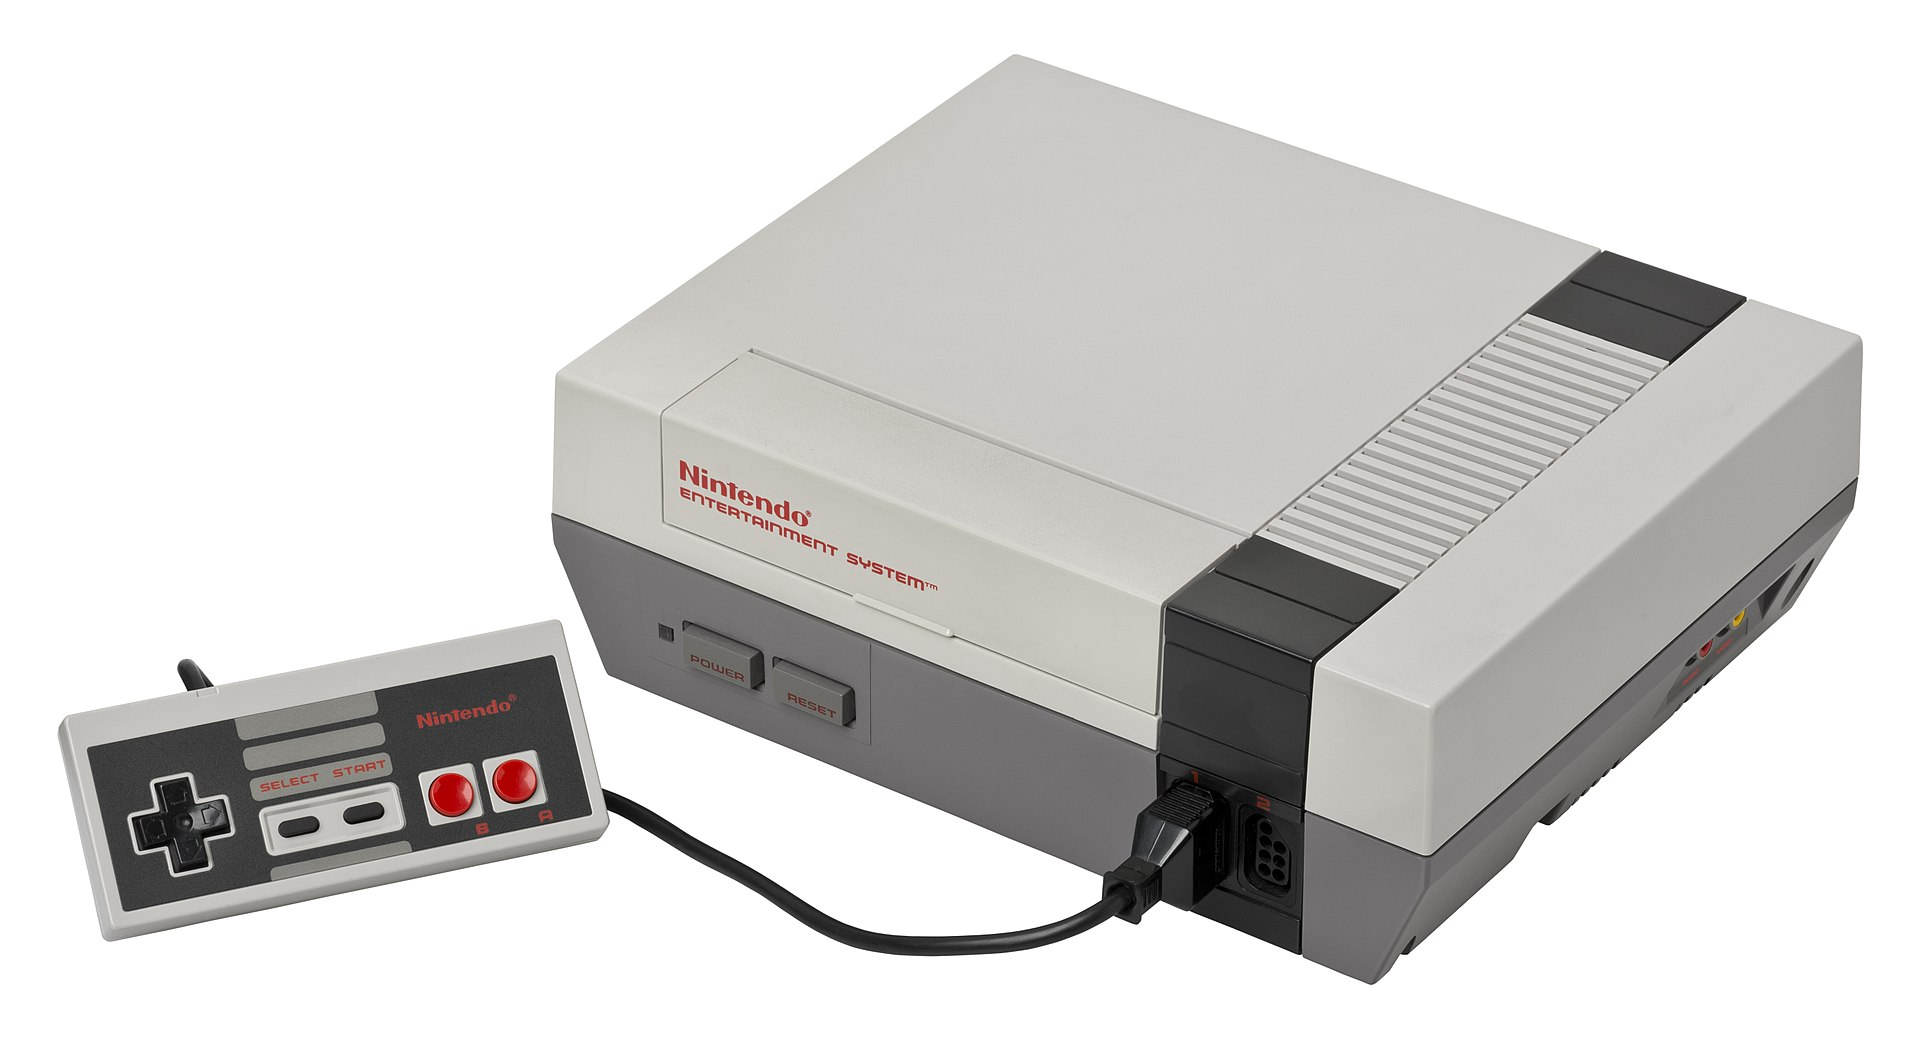
\includegraphics[scale=0.13]{nes.jpg}
	\caption{Nintendo Entertainment System (1985)}
	\label{fig:nes}
\end{figure}

A program feladata a NES kazetták futtatása. A felhasználó grafikus felület segítségével kiválaszthatja a futtatni kívánt, iNES formátumú kazetta fájlt, majd annak betöltése után az emulátor belekezd a videókimenet előállításába. Bemeneti eszközként billentyűzet vagy kontroller használható. A futtatás során lehetőség van az emulátor állapotának fájlként való mentésére és betöltésére. Az emulációt többféle módon is befolyásolhatja a felhasználó, amikbe beletartozik a játék szüneteltetése, adott mennyiségű CPU utasítás végrehajtása, valamint a teljes képkockánként történő léptetés.

A programot azoknak ajánlom, akik egy letisztult kezelőfelülettel rendelkező, több platformon is elérhető NES emulátorral szeretnék játszani kedvenc játékaikat.

\section{Minimum rendszerkövetelmények}

\begin{description}
	\item[Processzor:] Intel Core 2 Duo E8400 @ 3.0 GHz
	\item[Videókártya:] NVIDIA Geforce 7300 SE vagy 
	\newline vagy más OpenGL/DirectX kompatibilis videókártya
	\item[Memória:] 2 GB DDR2 @ 800 MHz
	\item[Tárhely:] 150 MB
	\item[Operációs rendszer:] Linux, Windows
\end{description}

A program a fenti konfiguráción történő tesztelés során problémamentesen működött.

\section{Telepítés}

\begin{itemize}
	\item Windows: A programot egy telepítőfájl segítségével telepíthetjük.
	\item Linux:
	\begin{lstlisting}[language=bash]
	$ tar xvf pure-nes-1.0.tar.gz
	$ cd pure-nes-1.0
	$ ./configure
	$ make
	\end{lstlisting}
\end{itemize}

\section{Indítás}
\begin{itemize}
	\item Windows: Kattintsunk a program parancsikonjára a Start Menüben vagy az asztalon.
	\item Linux:
	\begin{lstlisting}[language=bash]
	pure-nes-1.0$ stack exec pure-nes
	\end{lstlisting}
\end{itemize}


\section{Kompatibilis kazetták}

A NES megtervezésekor fontos cél volt, hogy a konzol életciklusa hosszú legyen, de ezt nem volt könnyű gazdaságos módon elérni. Azt a megoldás találták ki, hogy a kazetta a játék mellett tartalmazzon speciális integrált áramköröket, amik igény szerint bővíthették a hardveres erőforrásokat. Ezeket Mapper-nek nevezzük. A későbbi játékok előszeretettel használták ki ezt a lehetőséget. A legtöbb speciális áramkör a megnövelt ROM kezeléséhez volt szükséges, de akadt olyan is, amelyik további hangcsatornákat adott hozzá a hangfeldolgozó egységhez. Az emulátorom jelenleg a 0 és 2 típusú Mapper-eket támogatja, ezáltal 351 játékot képes elindítani.      

\section{Főmenü}

\begin{center}
	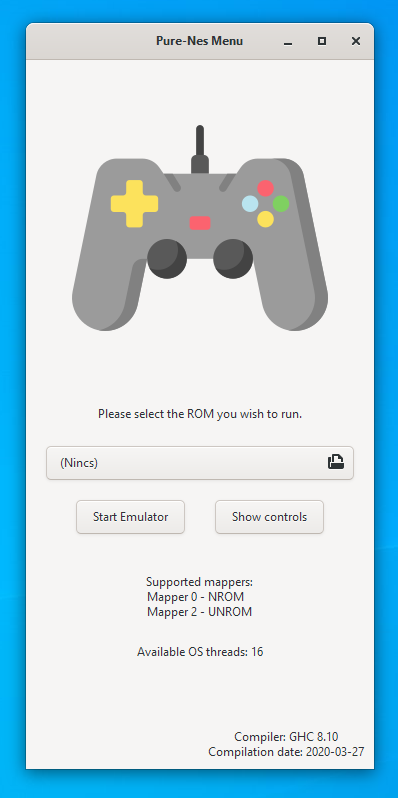
\includegraphics[scale=0.7]{menu.png}
\end{center}

\subsection{Kazetta kiválasztása}

A fájlkiválasztó segítségével adjuk meg a futtatni kívánt kazettát vagy mentést, majd nyomjunk a \emph{Start Emulator} gombra.
A program hibaüzenettel jelzi, ha a kazetta nem kompatibilis vagy a fájl formátuma nem megfelelő.

\subsection{Irányítási beállítások megtekintése}

A főmenü \emph{Show controls} gombjára kattintva megtekinthetjük a gombhozzárendeléseket.

\section{Játék alatt elérhető funkciók}

\subsection {Irányítás}

\begin{table}[H]
	\centering
	\begin{tabular}{ | l |  l | l | }
		\hline
		Virtuális kontroller & Billentyű & Joystick \\
		\hline			
		A & 1 & 2. gomb \\
		B & 2 & 3. gomb \\
		Select & 3 & 0. gomb \\
		Start & 4 & 1. gomb \\
		Up    & Fel nyíl & DPad Fel \\
		Down  & Lefele nyíl & DPad Le \\
		Left  & Balra nyíl & DPad Bal \\ 
		Right & Jobbra nyíl & DPad Jobb \\
		\hline
	\end{tabular}
	\caption{Játékok irányításához használt gombok}
	
	\begin{flushleft}
		A Joystick vezérlők gombkiosztása el szokott térni, ami azt jelenti, hogy a fizikailag ugyanott található gomboknak más az azonosítója. A felhasználó feladata, hogy szükség esetén egy másik programmal módosítsa eszközének kiosztását úgy, hogy az megegyezzen az emulátor szerint elvárttal.
	\end{flushleft}
	
	\begin{tabular}{ | l | c | }
		\hline
		Emulátor funkció & Billentyű \\
		\hline			
		Teljes képernyős nézet ki/be & R \\
		Szüneteltetés ki/be & Space \\
		100 processzor utasítás végrehajtása szüneteltetett állapotban & C \\
		A következő képkocka kiszámolása szüneteltett állapotban & F \\
		\hline
	\end{tabular}
	\caption{Az emuláció vezérlése}
\end{table}


\subsection{Mentési mappa kiválasztása}

A felhasználónak ki kell jelölnie egy mappát, amit a program a mentések kezelésére használ. A program hibaüzenetet ad, ha enélkül próbálunk menteni vagy gyors betöltést végrehajtani.

\subsection{Mentés}

A mentések a virtuális gép teljes állopata mellett a praktikusság érdekében a játék másolatát is tartalmazzák, tehát egy mentés betöltéséhez nem kell megőrizni a játék eredeti példányát.

\begin{center}
	
\includegraphics[scale=0.75]{save.png}
\end{center}

\subsubsection{Gyors mentés}

A gyors mentési funkcióval egy gombnyomásra elmenthetjük állásunkat. A mentés \emph{quick.purenes} néven jön létre a mappában. Ha már létezik ilyen fájl, az felül lesz írva.
Mentés létrehozása: \textbf{Quick Save} gomb vagy \textbf{F5} billentyű.
A mentés sikerességét egy pipa vagy kereszt jelzi a kezelőfelületen a mentés ikon mellett.
Ha a kontroller rendelkezik rezgőmotorral, akkor a sikeres mentés rezgéssel is jelezve lesz.

\subsubsection{Egyedi mentés létrehozása}

Adhatunk nevet a mentéseknek, ehhez írjuk be a nevet a szövegmezőbe és nyomjunk a \emph{Save} gombra. A mentés \emph{\{név\}.purenes} néven jön létre a mappában. A \emph{quick} nevet nem adhatjuk a mentésnek.

\subsection{Betöltés}

\begin{center}
	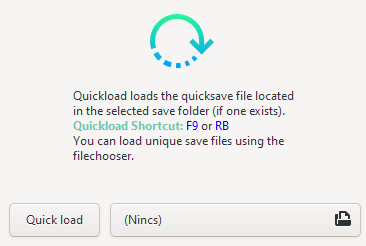
\includegraphics[scale=0.75]{load.png}
\end{center}

\textbf{Figyelem:} Mindkét betöltési módnál az aktuális munkamenet elveszik. Ha ezt el szeretnénk kerülni, akkor mentsünk előtte.

\subsubsection{Gyors betöltés}

A gyors betöltési funkció játék közben érhető el, miután kiválasztottuk a mentéseket tároló mappát. A \textbf{Quick load} gombbal, vagy az \textbf{F9} billentyűvel visszatölthetjük a korábban létrehozott gyorsmentést.
A betöltés sikeressége a mentéshez hasonló módon jelenik meg a kezelőfelületen.
A sikeres betöltést szintén rezgés fogja követni.

\vspace{0.2cm}
\textbf{Lehetséges hibaüzenet}
\begin{itemize}
	\item A kiválasztott mappában nem található gyorsmentés.
	Megoldás: hozzunk létre egy gyorsmentést.
\end{itemize}

\subsubsection{Egyedi mentés betöltése}

A fájlkiválasztó segítségével válasszuk ki a betölteni kívánt mentést.

\subsection{A játék megállítása}

A játék futása bármikor felfüggeszthető a \emph{Pause} gombbal, majd ezután folytatható a \emph{Resume} gombbal.

\begin{center}
	
\includegraphics[scale=0.8]{pause.png}
	\qquad
	
\includegraphics[scale=0.8]{resume.png}
\end{center}

\subsection{Visszatérés a főmenübe}
A \emph{Return To ROM selection} gomb bezárja a játékot és a felhasználói felületen visszanavigál minket a főmenübe.
\newline \textbf{Figyelem:} Az állásunk elveszik, ha előtte nem mentünk. 
\vspace{0.3cm}
\begin{center}
	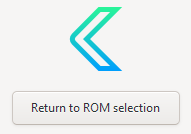
\includegraphics[scale=0.8]{return.png}
\end{center}

\subsection{Képernyőképek}
\vspace{0.5cm}
\begin{figure}[H]
	\centering
	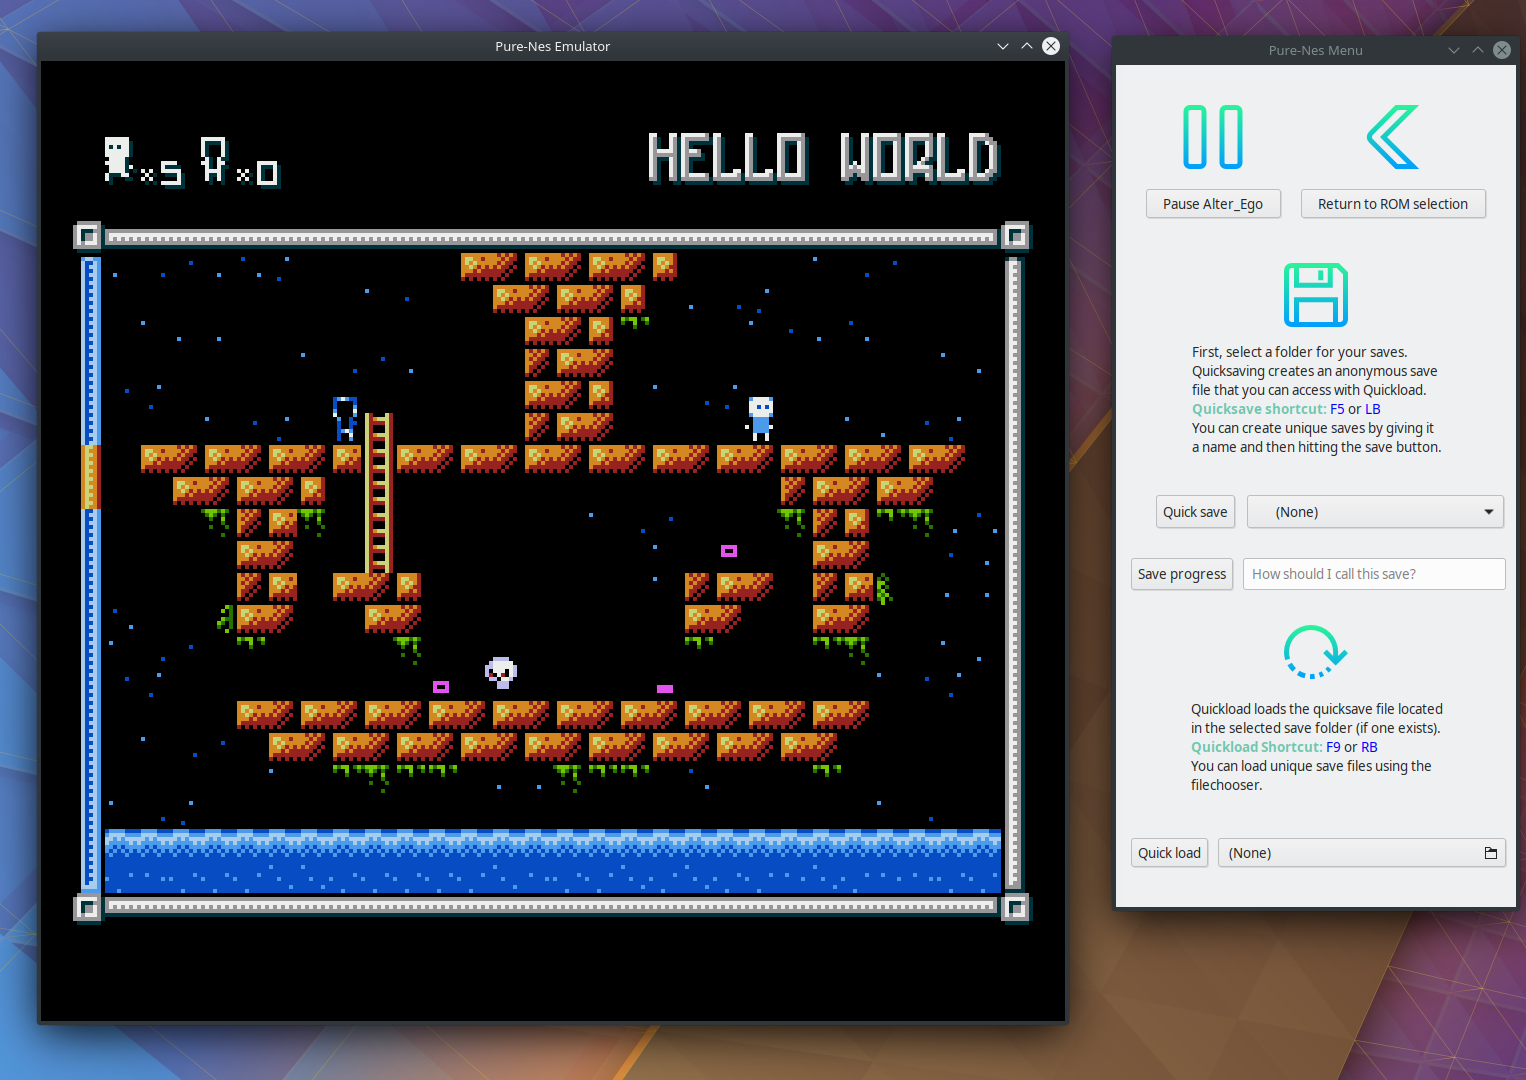
\includegraphics[scale=0.3]{shiru.png}
	\caption{Alter Ego by Shiru}
	\vspace{1cm}
	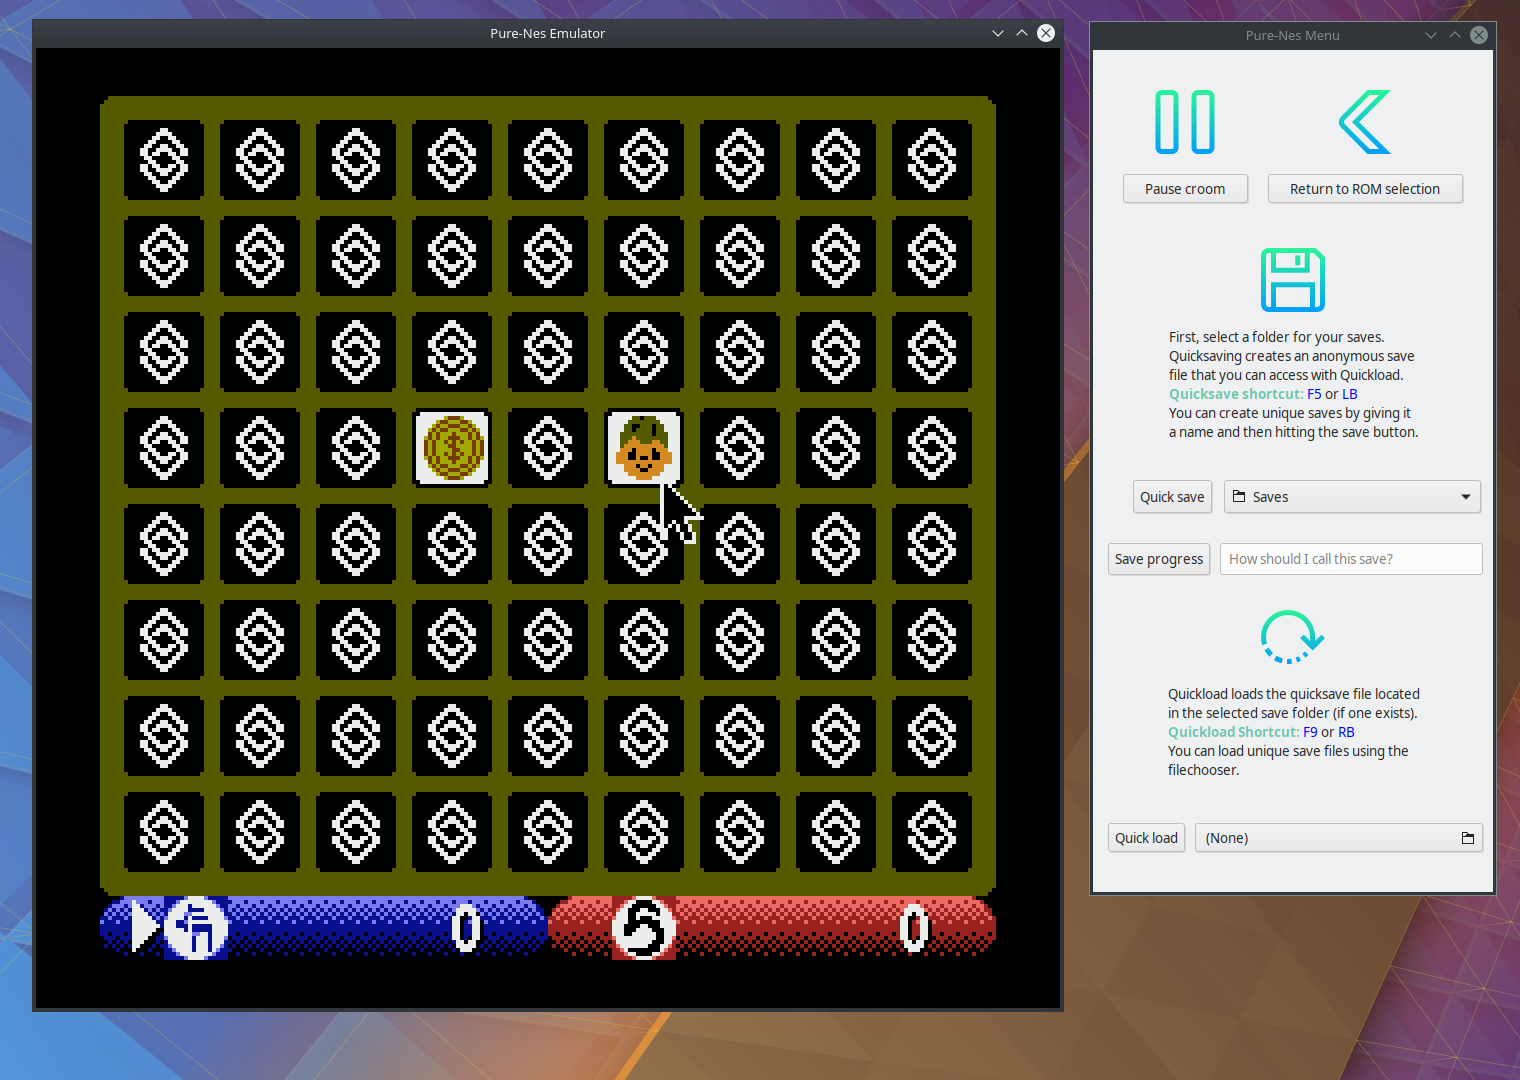
\includegraphics[scale=0.3]{croom.png}
	\caption{Concentration Room by Damian Yerrick}
\end{figure}
\cleardoublepage

\chapter{Fejlesztői dokumentáció} % Developer guide
\label{ch:impl}

\section{A NES felépítése}

\begin{figure}[H]
	\centering
	\includegraphics[scale=0.22]{mobo.jpg}
	\caption{A NES alaplapja}
\end{figure}

A NES emulációjához a következő komponenseket kell megismernünk és megvalósítanunk:

\begin{compactdesc}
	\item[Ricoh RP2A03:] 
	\hfill \\
	A hangchipet és központi feldolgozóegységet (CPU) tartalmazó integrált áramkör. Utóbbi nem más, mint az Apple II-ben és Commodore 64-ben használt 8-bites MOS Technology 6502.
	\item[Ricoh RP2C02:]
	\hfill \\
	A képfeldolgozó egység, rövid nevén PPU (Picture Processing Unit).
	\item[NROM és UNROM:] 
	\hfill \\
	Az emulátor által támogatott két kazettatípus integrált áramkörei.
	\item[Sztenderd NES kontroller:] 
	\hfill \\
	A konzol alapértelmezett beviteli eszköze.
\end{compactdesc}

\section{Órajel-frekvenciák}
A párhuzamosan működő komponenseket az órajelek hangolják össze. Az órajel-frekvencia határozza meg, hogy egy másodperc alatt hány atomi műveletet végez el egy komponens.
Minden komponens rendelkezik egy saját órajelfrekvenciával, amit egy központi órajelből származtatnak.

\begin{itemize}
	\item Központi órajel-frekvencia: $ f = \frac{236.25\;MHz}{11} \sim 21.477272\; MHz $
	\item CPU órajel-frekvencia: $ \frac{f}{12} \sim 1.789773 \; MHz  $
	\item PPU órajel-frekvencia: $ \frac{f}{4}  \sim 5.369318 \; MHz $
\end{itemize}

\section{A központi feldolgozóegységhez kapcsolódó fogalmak}

\begin{note}
	A hexadecimális értékeket \textbf{\$} prefix-el jelölöm.
\end{note}

\subsection{Opkód} 
Egy opkód a 6502 esetében csupán egyetlen bájt, amiből az utasításdekódoló egyértelműen meg tudja határozni a végrehajtandó utasítást és annak címzési módját.
Ezt a hozzárendelést az opkódmátrix írja le. Az emulációhoz emellett azt is tárolni kell az opkódmátrixban, hogy a végrehajtandó művelet hány központi órajel alatt fejeződik be, ugyanis csak ennek ismeretében tudjuk a CPU-t és a PPU-t precízen egymáshoz szinkronizálni.

\begin{figure}[H]
	\centering
	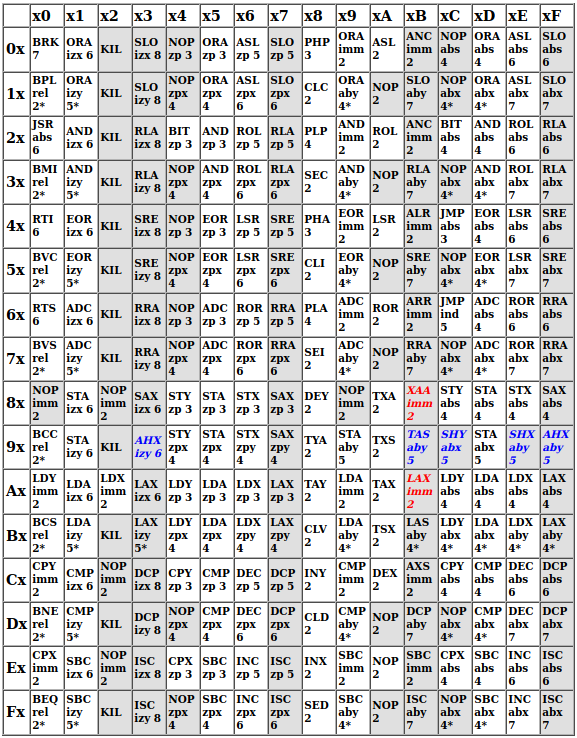
\includegraphics[scale=0.65]{opcodes.png}
	\caption{A 6502 opkódmátrixa}
	\label{fig:opcodes}
\end{figure}

Ha meg szeretnénk találni egy adott opkódhoz a hozzá tartozó információt, akkor szükségünk lesz az opkód hexadecimális alakjára, ami legfeljebb kétszámjegyű lehet. A nagyobb helyiértékű számjegy a keresett cella sorát, a kisebbik pedig az oszlopát írja le. Példaként a \ref{fig:opcodes} ábrán láthatjuk, hogy a \textbf{\$30} opkódhoz a BMI utasítás tartozik relatív címzéssel.
Azok az opkódok csillaggal vannak jelölve, amiknek a futási ideje megnőhet az aktuális argumentumoktól függően.
A szürkével jelölt opkódokhoz hivatalosan nincs utasítás rendelve. 
Ezeket a nem dokumentált, ``illegális'' opkódokat a processzor későbbi 
verzióinak hagyták fent. A tervezők nem tiltották meg azonban ezeknek a használatát, 
egyszerűen csak nem definiálták a viselkedésüket. Ennek ellenére több olyan illegális opkód is belekerült a dizájnba, ami később hasznosnak bizonyult. A játékfejlesztők próbálkozások útján
felfedezték, hogy melyek azok az opkódok, amiknek a viselkedése determinisztikus és néhány speciális feladat esetén érdemes őket használni.
Ritka ugyan, de van olyan játék, ami ezeket az opkódokat is használja, ezért ezeknek az opkódoknak az emulációját is megvalósítottam.

\subsection{Regiszterek}
A regiszter a processzor leggyorsabban elérhető memóriája.
A gyártási költségek alacsonyan tartása végett csak 6 regiszter került a processzorba.
Minden regiszter mellett zárójelben fel van tüntetve annak mérete bitekben megadva.

\begin{compactdesc}
	\item[A (8):] Akkumulátor, az aritmetikai műveletek eredményei ebbe kerülnek.
	\item[X (8) és Y (8):] 
	Index regiszterek, indirekt címzésnél használjuk őket.
	Ciklusok esetén a ciklusváltozót érdemes ezekben tárolnunk.
	\item[S (8):] 
	Verem mutató. A verem tetejének a kezdőcímtől vett eltolását tárolja.
	\item[P (8):]
	Státusz regiszter, ami 7 darab flag bitet tárol.
	\item[PC (16):]
	Programszámláló. 
	A következő opkód memóriacímét tárolja.
	Méretéből következik, hogy a processzor teljes címtartománya 64 KiB nagyságú.
\end{compactdesc}


\subsection{Memórialap}
Az $i$. lap egy 256 bájtos egybefüggő memóriarész, ami a $ [i \cdot \$100, \: (i+1) \cdot \$100) $ címtartományon helyezkedik el.

\subsection{Hívási verem}
Az egymásba ágyazott eljárásokat a processzor hardveresen támogatja, amihez egy vermet használ.
A verem az 1. lapon található, és a kisebb címek felé nő.
Eljárás hívásakor a verem tetejére kerül az aktuális programszámláló értéke, 
visszatéréskor pedig a veremről levett címre állítjuk be a programszámláló értékét.

\subsection{Megszakítás}
A komponensek kommunikációjának egyik módja a hardveres megszakítás.
A 6502 chip egy darab maszkolható \emph{(IRQ)} és egy nem maszkolható \emph{(NMI)} megszakítási lábbal rendelkezik.
A megszakítási vektorokkal a program beállíthatja, hogy egy bizonyos megszakításra milyen szubrutinnal kíván reagálni. A vektorok 2 bájtos tárolók, amik a kezelő szubrutin címét tartalmazzák. Az NMI-hez tartozó vektor a \$FFFA és a \$FFFB címeken, míg az IRQ-hoz tarozó vektor az \$FFFE és a \$FFFF címeken található. A 6502 ``kicsi az elején'' bájtsorrendű (little-endian) processzor, ezért a címeknek mindig az alsó 8 bitjét tárolja az alacsonyabb címen, a felső 8 bitjét pedig a magasabb címen.
A program dönthet úgy, hogy a maszkolható megszakítást figyelmen kívül hagyja (a kezelő szubrutin nem hívódik meg), ehhez az \emph{IRQ Disable} flag-et be kell állítania a státusz regiszterben. A nem maszkolható megszakítás esetén erre nincsen lehetőség, a végrehajtás mindenképpen a kezelő szubrutinhoz ugrik.
A nem maszkolható lábhoz a képfeldolgozó, a maszkolhatóhoz a hangchip van kötve.

\subsection{Opkód argumentum helye, fajtája}

\begin{figure}[H]
	\centering
	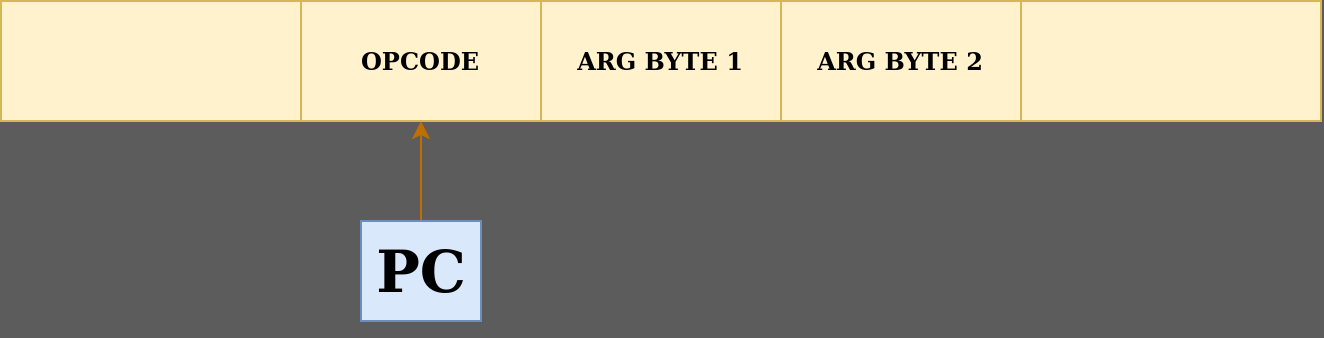
\includegraphics[scale=0.25]{opcode.png}
	\caption{Opkód argumentumainak helye}
	\label{fig:argplacement}
\end{figure}

A \ref{fig:argplacement} ábra szemlélteti, hogy az opkód argumentumok közvetlenül az opkód mögött, a \emph{PC+1} és \emph{PC+2} címeken helyezkedhetnek el a memóriában. Címzési módtól függően változhat az argumentumok száma 0, 1 és 2 bájt között.
Ha az opkód rendelkezik argumentummal vagy argumentumokkal, akkor azok a következő fajtájúak lehetnek:

\begin{compactitem}
	\item 2 bájt, ami abszolút memóriacímet ábrázol kicsi-az-elején bájtsorrenddel 
	\item 1 bájt, ami relatív eltolást ír le
	\item 1 bájt, ami a művelet közvetlen operandusa
\end{compactitem}

\subsection{Címzési módok}

Egy opkód után azoknál a címzési módoknál áll argumentum, amiknél a művelet elvégzéséhez 
szükséges operandus nem regiszterben, hanem a memóriában van. A címzési módok azt határozzák meg, hogy az argumentumból hogyan kell kiszámolni az operandus effektív 16 bites memóriacímét. Az alábbiakban felsorolt  címzési módoknál a zárójelben az opkódmátrixbeli név (amennyiben van) és az argumentum bájtok száma található.  


\begin{description}
	\item[Akkumulátor mód (0):] nincs argumentum, az utasítás az \textbf{A} regiszter értékét módosítja.
	\item[Azonnali mód (imm, 1):] az utasítás operandusa maga az argumentum. Jele: \#
	\newline
	Példa: az LDA \#\$0 utasítás nullára állítja az \textbf{A} regisztert.
	\item[Abszolút mód (abs, 2):] az argumentum az operandus effektív címe.
	\item[0. lap mód (zp, 1):] A CPU kevés regiszterét azzal ellensúlyozták, hogy ennek a speciális módnak köszönhetően a nulladik lapot hatékonyabban lehet címezni, mint a többit. 
	Mivel a 0. lap mérete 256 bájt, ezért teljes cím helyett elég egyetlen bájt a címzéséhez.
	A kisebb paraméter gyorsabban beolvasható és egyúttal a kódméretet is csökkenti.
	\item[Indexelt 0. lap mód (zpx, zpy, 1):]
	Hasonlóan most is csak a 0. lapot tudjuk címezni, de az argumentumhoz hozzáadjuk valamelyik index regiszter értékét.
	Az operandus címének kiszámítása: $ (arg1 + index) \mod 256 $
	\item[Indexelt abszolút mód (abx, aby, 2):] Az argumentumok egy teljes memóriacímet alkotnak, amihez hozzáadjuk a megadott index regiszter értékét. 
	\item[Implicit mód (0):] nincs szükség argumentumra, mert az utasítás regiszterekkel dolgozik.
	\item[Relatív mód (rel, 1):] Az elágazási utasítások használják ezt a címzési módot. Elágazásoknál ha a feltétel teljesül, akkor az argumentummal el kell tolni a programszámlálót. Az elágazási utasítások feltételeit lásd az \emph{\nameref{instructionset}} szekcióban.
	\item[Indirekt mód (ind, 2):] 
	Erre a címzési módra a JMP utasításnál van szükség.
	A két argumentum bájt együtt egy teljes memóriacímet alkot, legyen ez \emph{m}.
	Az operandus címét az \emph{m} és \emph{m+1} címeken találjuk, így tehát az operandus értékét a következő módon kapjuk meg: $$ operand := read(\;(read(m+1) << 8) \;\; | \;\; read(m)\;) $$
	\item[Indexelt indirekt mód (izx, 1):]
	Az X regisztert összeadjuk az argumentummal, így egy 0. lapon található címet kapunk.
	Erről a címről kell az operandus effektív címét kiolvasni.
	\begin{figure}[H]
		\centering
		\vspace{0.4cm}
		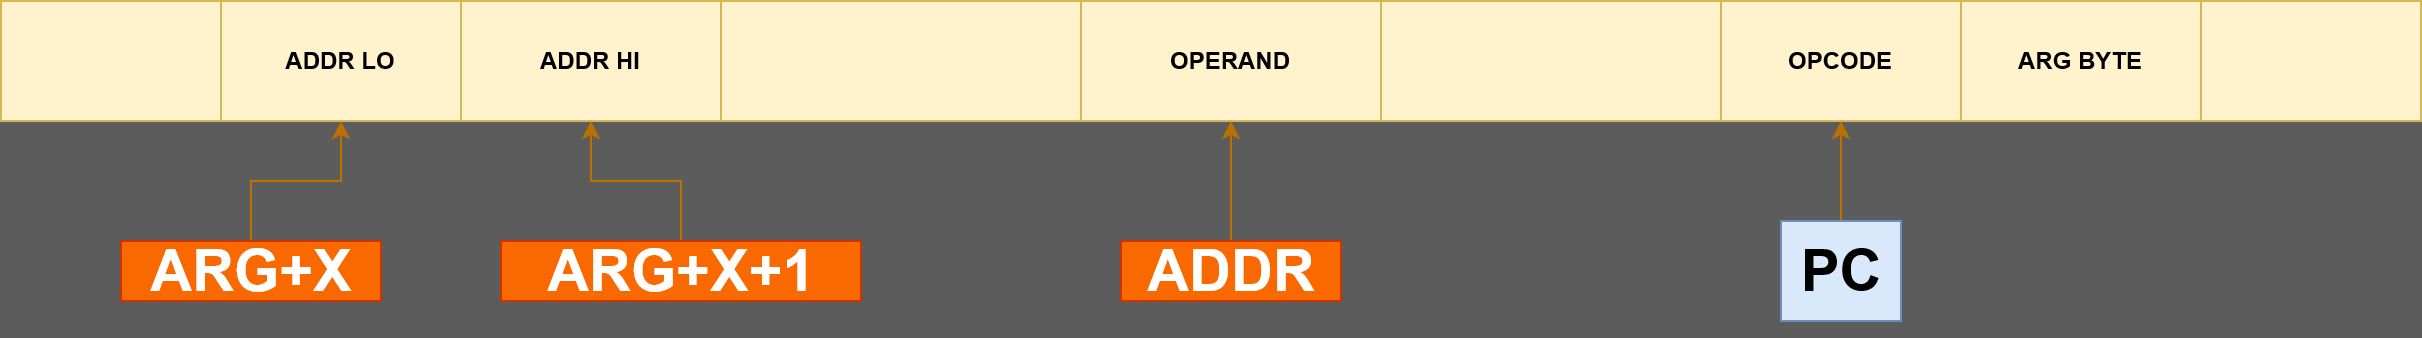
\includegraphics[width=1.1\textwidth,height=70px]{indexed_indirect.png}
		\caption{Indexelt indirekt címzés}
	\end{figure}
	\item[Indirekt indexelt mód (izy, 1):]
	Az argumentum egy 0. lapon található címre mutat, amit ha összeadunk az Y regiszter értékével, akkor megkapjuk az operandus effektív címét. 
	
	
	
\end{description}

Az \textbf{abx}, \textbf{aby} és \textbf{izy} indexelt címzési módok és bizonyos utasítások kombinációjánál előfordulhat, hogy a végleges operandus cím és az indexelés előtt álló cím különböző memórialapra esik. Ebben az esetben 1 órajelciklussal tovább tart az utasítás végrehajtása.
Emellett az elágazási utasítások (relatív címzés) több ciklus alatt fejeződnek be, ha az ugrási feltétel teljesül. Ha az ugrás előtti PC értéke és az ugrási cél más lapra esik, akkor +2, ellenkező esetben csak +1 órajelciklussal kell számolni.

\subsection{Memóriatérkép}

A memóriatérkép leírja a címtér felosztását a komponensek között.
A memóriatérképből meg tudjuk állapítani, hogy egy adott címen található bájt kiolvasásához vagy írásához melyik komponens hardveres logikáját kell alkalmazni.

\begin{table}[H]
	\centering
	\begin{tabular}{ | l | l | }
		\hline
		Tartomány & Eszköz \\
		\hline			
		$ \$0000 - \$07FF $ & CPU RAM \\
		$ \$0800 - \$1FFF $ & CPU RAM tükrözése \\
		$ \$2000 - \$2007 $ & PPU regiszterek \\
		$ \$2008 - \$3FFF $ & PPU regiszterek tükrözése \\
		$ \$4000 - \$4017 $ & APU és IO regiszterek \\
		$ \$4018 - \$401F $ & APU és IO regiszterek tükrözése \\
		$ \$4020 - \$FFFF $ & Kazetta \\
		\hline
	\end{tabular}
\end{table}

\subsection{Memóriatükrözés}
Memóriatükrözésről beszélünk, amikor fizikailag ugyanazt a memóriaterületet több memóriacímről is el tudjuk érni. Ha egy címtartomány $x$ bájtonként tükrözve van, akkor minden olyan $a$ és $b$ memóriacím ugyanarra a bájtra mutat, ami a tartományba vagy a tükrözésébe esik és $a \equiv b\ (\textrm{mod}\ x)$.  A CPU RAM 2 KiB-onként tükrözve van, amiből következik, hogy a \textbf{\$0001}, \textbf{\$0801} \textbf{\$1001}, \textbf{\$1801} címek ugyanarra a bájtra mutatnak. Egy címtartomány tükrözése lehet nagyobb mint az eredeti tartomány (például a CPU RAM esetében a tükrözési tartomány háromszor nagyobb).

\subsection{Státusz flagek}

\begin{compactenum}
	\setcounter{enumi}{-1}
	\item bit: C = Carry \newline Összeadások, forgatások, eltolások során a leeső biteket jelzésére.
	\item bit: Z = Zero   \newline Aritmetikai művelet eredménye vagy mozgatott bájt 0.
	\item bit: I = IRQ Disable
	\newline Az 1-re állításával maszkoljuk az IRQ-t.
	\item bit: D = Decimal mode
	\newline
	A NES nem használja ezt a flag-et.
	\item bit: B = BRK Command
	\newline Az 1-re állításával generálhatunk egy szoftveres megszakítást. 
	\setcounter{enumi}{5}
	\item bit: V = Overflow
	\newline 
	Aritmetikai műveleteknél a túlcsordulás vagy alulcsordulás jelzésére.
	A BIT utasítás speciálisan használja.
	\item bit: N = Negative
	\newline A manipulált bájt negatív, vagyis a legnagyobb helyiértékű bitje 1.
\end{compactenum}

\subsection{Utasításkészlet}
\label{instructionset}

\begin{compactdesc}
	\item Aritmetikai és logikai egység (ALU)
	\begin{compactdesc}
		\item[ADC:] Összeadás
		\item[SBC:] Kivonás
		\item[AND:] Logikai ÉS művelet
		\item[ASL:] Bájt balra elcsúsztatása
		\item[LSR:] Bájt jobbra elcsúsztatása
		\item[ORA:] Logikai VAGY
		\item[EOR:] Kizárásos VAGY
		\item[INC, INX, INY:] növelés eggyel
		\item[DEC, DEX, DEY:] csökkentés eggyel
		\item[ROL, ROR:] bájt forgatása
	\end{compactdesc}
	\item 
	Összehasonlítás, tesztelés
	\begin{compactdesc}
		\item[CMP, CPX, CPY:]  \hfill \\ A megadott címen található bájt és rendre az A, X és Y regiszterekben található bájt között az $=$ és a $>=$ reláció kiértékelése
		\item[BIT:] Az operandus bájt maszkolása (\&) az A regiszter tartalmával, az eredmény szerint a Z,N,V flag-ek frissítése 
	\end{compactdesc}
	\item Veremműveletek
	\begin{compactdesc}
		\item[PHA:] Az akkumulátor regiszter értékének felrakása a veremre 
		\item[PHP:] A státusz regiszter értékének felrakása a veremre
		\item[PHA:] Az akkumulátor regiszter új értékének levétele a veremről
		\item[PHP:] A státusz regiszter új értékének levétele a veremről
	\end{compactdesc}
	\item Vezérlés
	\begin{compactdesc}
		\item[JMP:] Vezérlés áthelyezése egy megadott memóriacímhez, avagy a programszámláló átállítása erre a címre
		\item[JSR:] Szubrutin hívás (visszatérési cím elmentése + \textbf{JMP})
		\item[RTS:] Visszatérés szubrutinból (visszatérési cím kiolvasása + \textbf{JMP})
		\item[BRK:] Szoftveresen generált megszakítás
		\item[RTI:] Visszatérés megszakításkezelőből
	\end{compactdesc}
	\item Flag manipuláció (a utasításnév harmadik betűje a változtatott flag-et jelöli) \newline \textbf{CLC, CLD, CLI, CLV, SED, SEC, SEI}
	\newline
	(C = Clear, S = Set)
	\item Elágazások: vezérlés áthelyezése akkor, ha teljesül a feltétel az utasítás által vizsgált státusz flag-re
	\newline \textbf{BCC(C=0), BCS(C=1), BNE(Z=0), BEQ(Z=1), BPL(N=0), BMI(N=1),  BVC(V=0), BVS(V=1)}
	\item Bájtok mozgatása regiszterek és a memória között
	\newline
	\textbf{LDA, LDX, LDY, STA, STX, STY} 
	\newline
	(L = Load, S = Store)
	\newline
	A név harmadik betűje a használt regisztert jelöli.
	\item Bájtok mozgatása regiszterek között
	\newline
	\textbf{TAX, TAY, TSX, TXA, TXS, TYA}
	\newline
	A név második betűje a forrásregisztert, a harmadik a célregisztert jelöli.
\end{compactdesc}

\section{Kazetták}

A kazettákon logikai szempontból kétfajta memória található: PRG és CHR.
A PRG jellemzően csak olvasható memória (ROM), ahol a processzor által végrehajtandó utasítások, avagy a játéklogika kapott helyett. Mérete NROM esetében 16 KiB vagy 32 KiB, UNROM-nál pedig 64 KiB vagy 128 KiB. A 8 KiB méretű A CHR ROM/RAM memória, mely 8 KiB méretű és játék sprite-jait tárolja, amik 8*8 pixeles kis képekből állnak. Ezeket a kis képeket ezentúl alakzatoknak fogom hívni. 

\subsection{Az iNES fájlformátum}

Az iNES fájlformátumot egy korai NES emulátor vezette be a NES játékok bináris formában történő terjesztésére. A fájl elején található 16 bájtos fejléc többek között a mapper áramkör azonosítóját, a képfeldolgozó névtábláinak tükrözési módját, valamint a PRG ROM és a CHR memóriák típusát (ROM/RAM) és méretét határozza meg. A fejléc után ezek tartalma található.

\section{A képfeldolgozó egység}

\subsection{Színpaletta}

A képpontok végső RGB színkódjának meghatározása többféle módon is lehetséges. A gyors, de kevésbé pontos módszer, ha egy fix palettával dolgozunk. A paletta hozzárendel egy $\$0$ és $\$3F$ közötti azonosítóhoz egy színkódot, így tehát 55 különböző színt tudunk megjeleníteni. A lassabb, de pontosabb módszer, hogy az analóg NTSC videójelre történő konverziót is emuláljuk. Az emulátoromnál a gyorsabb módszert implementáltam.

\vspace{0.3cm}
\begin{figure}[H]
	\centering
	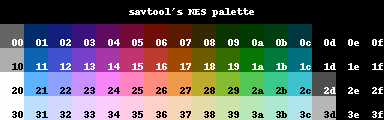
\includegraphics{palette.png}
	\caption{A 2C02 színpalettája}
\end{figure}

\clearpage

\subsection{Paletta indexek}

A $\$3F00 - \$3F1F$ címtartományon található paletta indexben kerülnek eltárolásra a használatban lévő színek színpalettabeli azonosítói, csoportokba (palettákba) rendezve. A hardveres limitációk miatt a hátteret 16x16 pixeles cellákra osztották fel. Egy cellán belül kizárólag 4 féle szín fordulhatott elő. Ezeket a 4 színből álló színkombinációkat kissé megtévesztő módon szintén palettáknak nevezik. További limitáció, hogy a paletták 4. színe nem változtatható, mert ezek mindig a \$3F00 címet (a háttérszínt) tükrözik.

\begin{table}[H]
	\centering
	\begin{tabular}{ | l | l | }
		\hline
		Tartomány & Paletta \\
		\hline			
		$ \$3F00 $ & Univerzális háttérszín \\
		$ \$3F01 - \$3F03 $ & 0. háttér paletta \\
		$ \$3F05 - \$3F07 $ & 1. háttér paletta \\
		$ \$3F09 - \$3F0B $ & 2. háttér paletta \\
		$ \$3F0D - \$3F0F $ & 3. háttér paletta \\
		$ \$3F11 - \$3F13 $ & 0. sprite paletta \\
		$ \$3F15 - \$3F17 $ & 1. sprite paletta \\
		$ \$3F19 - \$3F1B $ & 2. sprite paletta \\
		$ \$3F1D - \$3F1F $ & 3. sprite paletta \\
		\hline
	\end{tabular}
	\caption{A paletta RAM struktúrája}
	\label{fig:paletteram}
\end{table}

\subsection{Alakzattáblázat}

A CHR memóriában található két alakzattáblázat az alakzatokat tárolja egy speciális formátumban. Ha az alakzatokat úgy reprezentálnánk, hogy minden pixelre eltárolnánk egy színkódot, akkor pixelenként 6 bitre lenne szükségünk (mivel 55 színkódból választhatunk). Ehelyett pixelenként csak 2 bitet (egy szignifikáns és egy kevésbé szignifikáns bitet) tárolnunk, amik együtt egy, a palettaindexben található palettán belüli színt azonosítanak. Az attribútumtábla segítségével fogjuk később meghatározni, hogy a vizsgált pixelhez melyik paletta tartozik. Mivel a paletta index írható és olvasható memória is, így a program futási időben, dinamikusan változtathatja, hogy egy paletta milyen színeket tartalmaz, ezáltal pár lépésben átszínezheti az összes alakzatot, ami az adott palettát használja.
Egy alakzattáblázat 16x16 darab alakzatot tartalmaz és egy alakzat 8x8 pixeles, ebből adódóan a táblázat teljes mérete $16\cdot16\cdot(8\cdot8\cdot2)\div8 = 4096$ bájt. Egy alakzat pixeljeinek bitjeit $(8\cdot8\cdot2)\div8 = 16$ egymást követő bájt tárolja a \ref{fig:patt} ábrán szemléltetett módon. Először 8 bájton keresztül a kevésbé szignifikáns bitek, majd ezután újabb 8 bájton át a szignifikánsabb bitek helyezkednek el.

\begin{figure}[H]
	\centering
	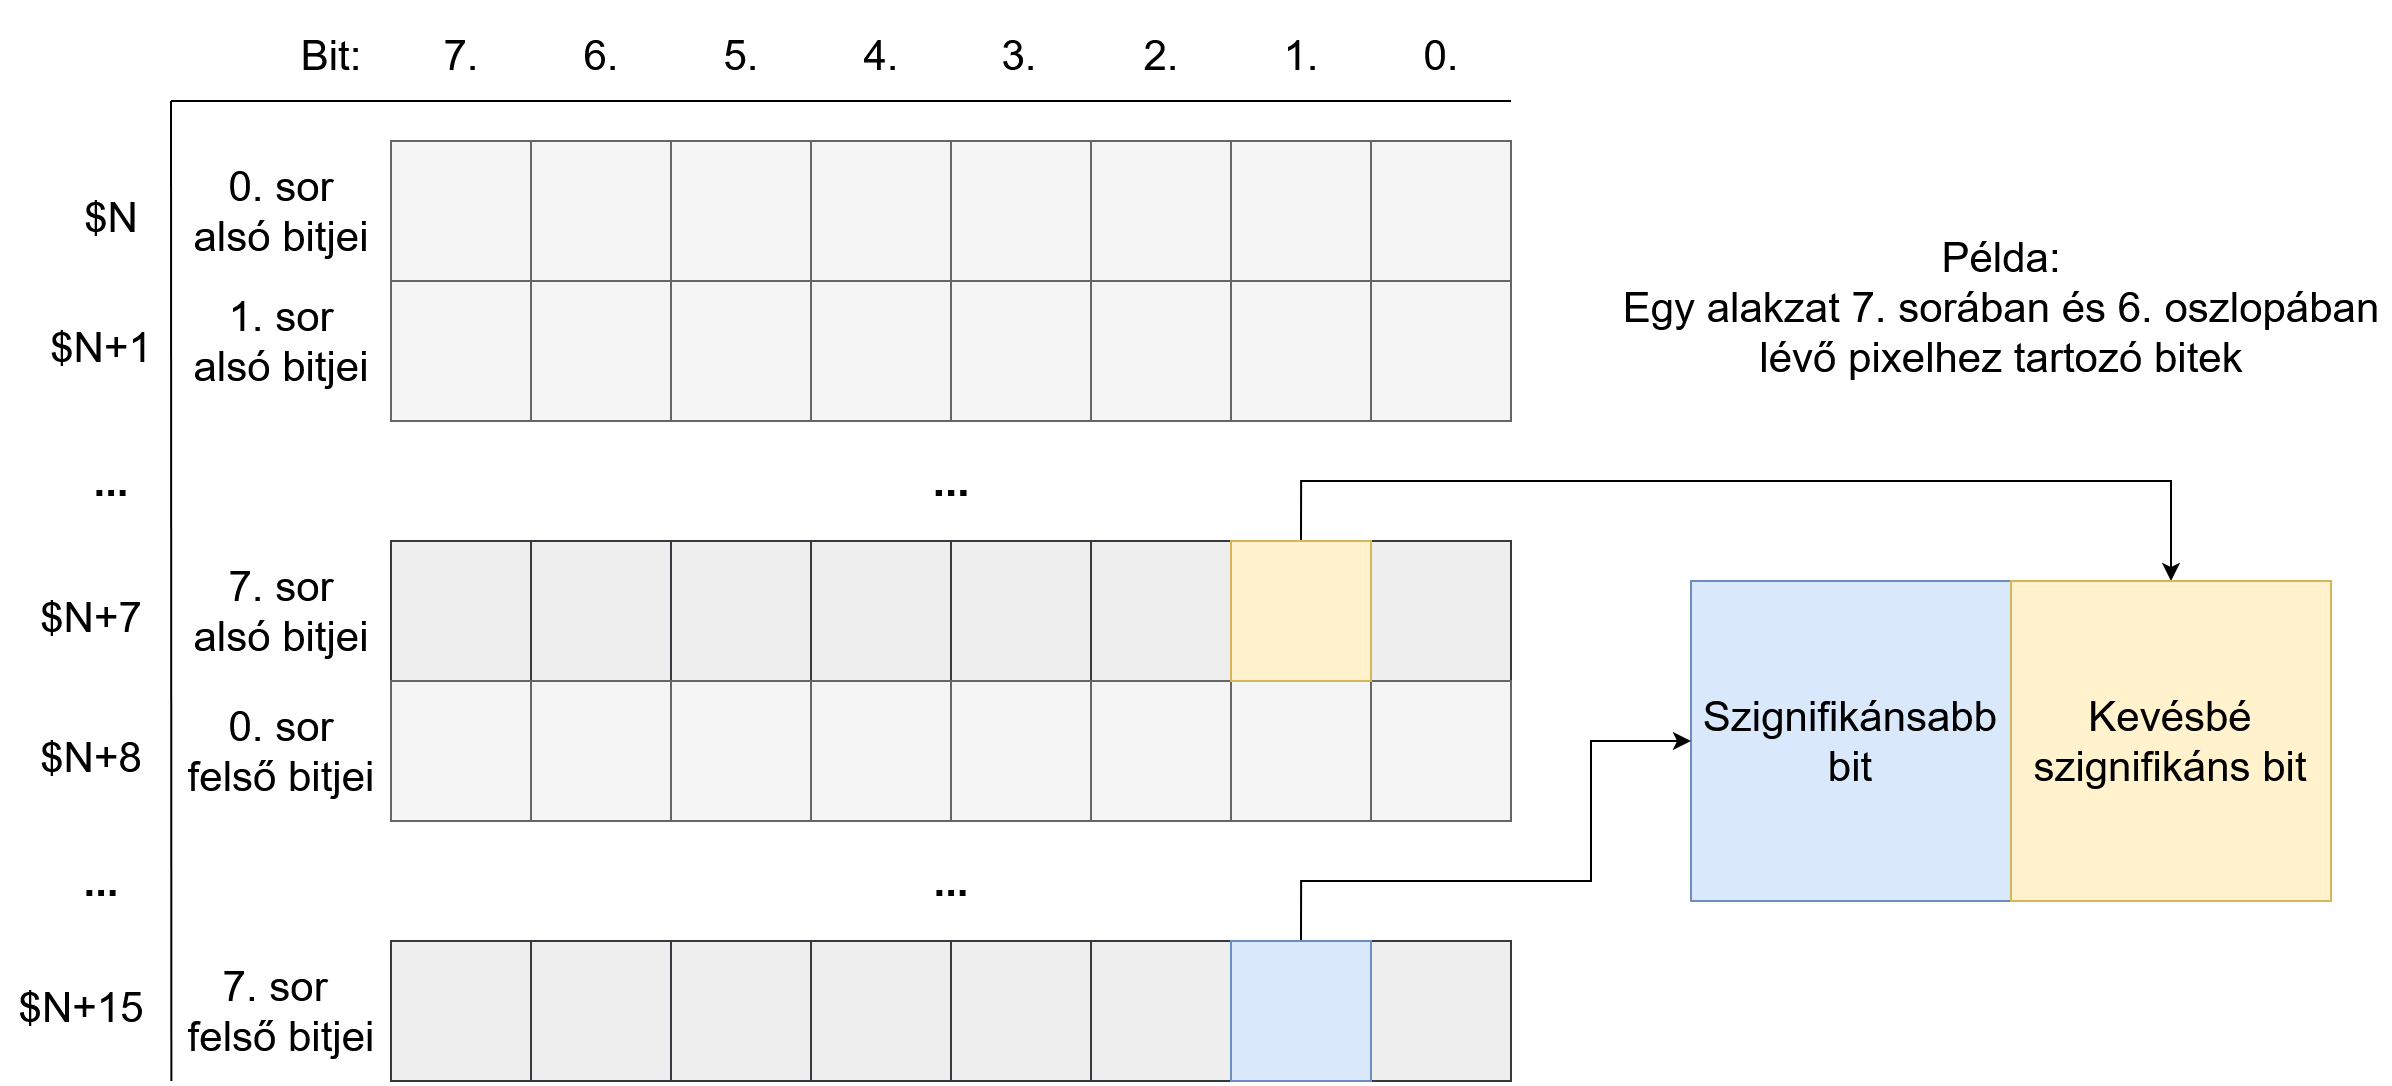
\includegraphics[scale=0.175,frame]{patt.png}
	\caption{Egy alakzat reprezentálása}
	\label{fig:patt}
\end{figure}


\begin{figure}[H]
	\centering
	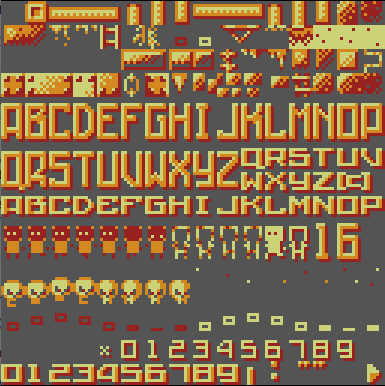
\includegraphics[width=0.45\linewidth,frame]{patt2.png}
	\hspace{5pt}
	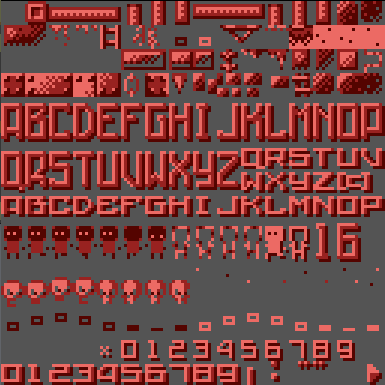
\includegraphics[width=0.45\linewidth,frame]{patt1.png}
	\caption{Az Alter Ego játék 0. alakzattáblázata különböző palettákkal kirajzolva}
\end{figure}

\subsection{Rétegek}
A képfeldolgozó két réteget képes kezelni hardveresen, ezek a háttér és a sprite rétegek.
Általában a képkocka azon részei tartoznak a háttérhez, amik ritkán változnak (például feliratok, számlálók, mozdulatlan képek) és a kirajzolásukhoz nem szükséges további transzformáció (eltolás, tükrözés). A háttérben az alakzatok 30 sorból és 32 oszlopból álló négyzetrácsot alkotnak (ebből és az alakzatok méretéből ered a NES 256*240 pixeles felbontása).
A háttér rétegben egyesével nem lehet alakzatokat eltolni, csak az egész háttér eltolása lehetséges. A sprite rétegben nagyobb flexibilitás áll rendelkezésre, ugyanis itt egyenként, pixel pontosságú eltolással, valamint horizontális és/vagy vertikális tükrözéssel rajzolhatjuk ki az alakzatokat. A sprite rétegnél legfeljebb 64 alakzat szerepelhet egy képkockán (ez a megkötés a később ismertetett OAM méretéből adódik).  

\subsection{Névtáblázat}

A háttérréteg négyzetrácsának elrendezését a névtáblázatok tárolják. A névtáblázat a háttér 960 darab alakzatcellájának mindegyikéhez eltárolja a cellába rajzolandó alakzat sorszámát. Ez a sorszám relatív, ugyanis mindig azon az alakzattáblázaton belül értendő, amit a CONTROLLER regiszterrel a program kiválasztott.

\subsection{Attribútum táblák}

Minden névtáblához tartozik egy 64 bájtos attribútumtáblázat, ahol minden bájt egy 4*4 alakzatcellából álló terület palettáit határozza meg. A bájtok 4 darab 2 bites részre vannak felosztva, ahol mindegyik rész egy 2*2 cellából álló terület palettájának sorszámát (0-3) kódolja el. Ennek a reprezentációnak a következménye, hogy a háttér 4 cellából álló csoportjai mindig egy palettán osztoznak.

A 16 cellát lefedő bájt a következőképpen van felosztva a 4 cellás területek között:

\begin{figure}[H]
	\centering
	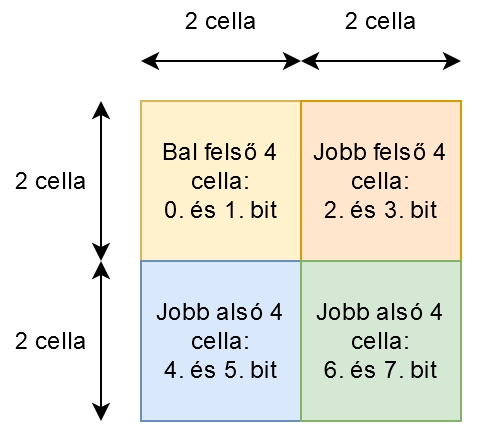
\includegraphics[width=0.4\linewidth]{attrtable.png}
\end{figure}


\subsection{Háttéreltolás}

A háttéreltolással pixelpontossággal megszabhatjuk, hogy a háttér mely része legyen látható a játékos számára.
Az eltolás miatt van szükség több névtáblára, ugyanis a lecsúszó háttérrész a valamelyik másik névtáblából lesz kiolvasva. 

\subsection{OAM (Object Attribute Memory)}

A sprite réteg elrendezését leíró 256 bájtos memória. 64 darab alakzatról tárol információt, amik a következők:

\begin{compactitem}
	\item X és Y koordináta
	\item A sprite réteg aktív alakzattáblázatán belüli sorszám
	\item Tükrözés
	\item Paletta sorszám
	\item Prioritás a háttérrel szemben
\end{compactitem}

\subsection{Regiszterek}

A CPU és a PPU az alább látható 9 darab egy bájtos regiszter segítségével tud egymással kommunikálni. A regisztereket a CPU a zárójelekben található címeken tudja elérni.
Az olvasató regiszterek \textbf{R}, az írhatók \textbf{W} betűvel vannak megjelölve.

\vspace{0.25cm}

\begin{description}
	\item[CONTROLLER(\$2000, W):] \hfill \\
	A kirajzolás vezérlésére szolgáló regiszter.
	Beállítható vele a következő képkockánál használandó táblázatok indexe.
	\begin{compactdesc}
		\item[0-1. bit:] Aktív névtáblázat indexe
		\item[2. bit:] VRAM cím inkrementálási mód
		\item[3. bit:] Aktív alakzattáblázat indexe a sprite rétegnél
		\item[4. bit:] Aktív alakzattáblázat indexe a háttér rétegnél
		\item[5. bit:] Sprite méret (8x8 vagy 8x16 pixel)
		\item[6. bit:] Az emuláció során nem használt bit
		\item[7. bit:] NMI generálása a PPU tétlen periódusának kezdetén
	\end{compactdesc}
	\item[MASK(\$2001, W):] \hfill \\
	A rétegek egyenkénti ki/bekapcsolása és speciális effektusok 
	(például szürkeárnyalat) vezérelhetők vele.
	\item[STATUS(\$2002, R):] \hfill \\
	A kirajzolás alatt bekövetkező eseményeket jelzi a PPU a CPU-nak ezzel a regiszeterrel.
	Ilyen esemény például a sprite túlcsordulás, ami akkor áll fent, ha több mint a 8 alakzat kerülne egy sorra a sprite rétegben. 
	\item[OAMADDR(\$2003, W) és OAMDATA(\$2004, R/W):] \hfill \\
	A processzor ezen két regiszter segítségével képes új adatokkal feltölteni az OAM memóriát.
	Az alábbi kódrészlet azt szemlélteti, hogy az \emph{adatok} tömb tartalmát hogyan kell a CPU memóriájából
	az OAM-ba átmásolni egy megadott címtől kezdve. Az OAMDATA írása után az OAMADDR automatikusan inkrementálódik a másolás gyorsításának érdekében.
	\begin{lstlisting}
	OAMADDR := 8 bites OAM cim
	for i in 1..adatok.hossz
		OAMDATA := adatok[i]
	\end{lstlisting}
	\item[PPUSCROLL(\$2005, W):] \hfill \\
	Beállíthatjuk vele, hogy a hátteret hány pixellel szeretnénk arrébbcsúsztatni (Horizontális tükrözésnél vízszintesen, vertikális tükrözésnél függőlegesen).
	\item[PPUADDR(\$2006, W) és PPUDATA(\$2007, R/W):] \hfill \\
	A névtáblák frissítésére szolgálnak. Hasonlóan kell őket használni, mint az OAMADDR és OAMDATA regisztereket.
	\item[OAMDMA(\$4014, W):] \hfill \\
	Az OAM memória frissítésének egy alternatív, gyorsabb módja a Direct Memory Access (DMA). Ekkor a processzorban található dedikált hardver másolja át az adatokat egyenesen a CPU RAM-ból az OAM memóriába. A másolás megkezdéséhez annak a memórialapnak a sorszámát kell beírni a regiszterbe, ahol az átmásolandó adatok találhatók.
\end{description}

\subsection{Memóriatérkép}

\begin{table}[H]
	\centering
	\begin{tabular}{ | l | l | }
		\hline
		Tartomány & Paletta \\
		\hline			
		$ \$0000 - \$0FFF $ & 0. Alakzattáblázat \\
		$ \$1000 - \$1FFF $ & 1. Alakzattáblázat \\
		$ \$2000 - \$23FF $ & 0. Névtáblázat \\
		$ \$2400 - \$27FF $ & 1. Névtáblázat \\
		$ \$2800 - \$2BFF $ & 2. Névtáblázat \\
		$ \$2C00 - \$2FFF $ & 3. Névtáblázat \\
		$ \$3000 - \$3EFF $ & A 0-3. névtáblázatok tükrözése \\
		$ \$3F00 - \$3F1F $ & Paletta indexek \\
		$ \$3F20 - \$3FFF $ & Paletta indexek tükrözése \\
		\hline
	\end{tabular}
	\caption{A képfeldolgozó memóriatérképe}
	\label{fig:ppumemmap}
\end{table}

\subsection{A háttér kirajzolásának egyszerű algoritmusa}

Ezen a ponton már minden részletet ismerünk ahhoz, hogy megérthessük a háttérkirajzolás logikáját. A következő pszeudokód azt szemlélteti, hogy a fent említett táblázatokat és a paletta indexet hogyan kell együtt használni a háttér kiszámolásához. Az egyszerűség kedvéért a háttéreltolást itt nem veszem figyelembe. Sajnos ez az algoritmus ebben a formában emulációra nem alkalmas, mert nehézzé teszi a processzor párhuzamos, megfelelő szinkronizációval történő futtatását.
\vspace{0.3cm}

\begin{lstlisting}

// Egy bájt indexedik bitjének kiolvasása (0/1)
byte bit(byte bájt, int index)
begin
	return (bájt >> index) & 1
end

// Az alábbi függvénnyel olvasunk a PPU címterében
byte olvas(cím)

type RGB_Kód = (byte, byte, byte)

// Az alábbi függvény a paletta index és a színpaletta felhasználásával 
// visszaadja, hogy egy adott sorszamú palettán belül az indexedik színnek mi
// az RGB kódja
RGB_Kód színKeresés(byte palettaSorszám, byte index)

// Az eredményül kapott pixeleket tároló kétdimenziós tömb
RGBKod pixelek[256][240]

procedure HáttérKirajzol
begin
	// A CONTROLLER regiszterrel a választott névtáblázat
	// és alakzattáblázat kezdőcímének meghatározása
	cím aktívNévtáblazat     := $2000 + (CONTROLLER & 0b11) * $400
	cím aktívAlakzatTáblázat := bit(CONTROLLER, 4) * $1000
	
	// Végigiterálás a háttér celláin
	for cellaSor in 0..29
		for cellaOszlop in 0..31
		begin
		  // A cellához tartozó névtáblabájt indexének kiszámolása
		  byte NTB_Eltolás := cellaSor * 32 + cellaOszlop 
		  
		  // A névtáblabájt kiolvasása
			byte NTB := olvas(aktivNevtabla + NTB_Eltolas)
			
			// A cellához tartozó attribútumbájt eltolása a névtábla
			// kezdőcíméhez viszonyítva.
			cím ATB_Eltolás := 
				// Átlépjük a 960 névtáblabájtot 
				$3C0 +		
								
				// Átlépjük az előző cellasorok attribútumbájtjait
				// Emlékeztető: egy sorban 32 alakzat van amik 
				// négyesével osztoznak a bájton
				(cellaSor div 4) * 8 + 	
					
				// Átlépjük a jelenlegi cellasorban az előző attribútumbájtokat
				(cellaOszlop div 4)         
				
			// Az attribútumbájt kiolvasása
			byte ATB := olvas(aktívNévtáblázat + ATB_Eltolás)
			
			// Az attribútumbájtnak a cellához tartozó 2 bites része lesz a palettasorszám.
			// Ki kell számolni, hogy a cella melyik (bal felső, jobb felső, stb.)
			// kvadránsába esik a bájt által lefedett 4*4-es területnek, ugyanis így
			// kapjuk meg, hogy a bájtot 0, 2, 4 vagy 6 bittel kell jobbra csúsztatni.
			byte kvadráns := (cellaSor & 0b10)*2 + (cellaOszlop & 0b10) 
			byte palettaSorszám :=
				(ATB >> kvadráns) & 0b11
				
			// Az alakzat kezdőcíme az alakzattáblában
			// Segítség: egy alakzat (8*8*2)/8 = 16 bájtot foglal
			cim alakzatCím := aktívAlakzatTáblázat + NTB*16
				
			// Végigiterálás a cella 8*8 pixeles területén
			for pixelSor in 0..7
			begin
				cim alakzatSor := alakzatCím + pixelSor
				
				// A sor alsó bitjei
				byte alakzatLSB = olvas(alakzatSor)
				
				// A sor felső bitjei		
				byte alakzatMSB = olvas(alakzatSor + 8)
				
				for pixelOszlop 0..7
				begin
					// A pixelhez tartozó 2 bittel a palettán belüli szín meghatározása
					byte palettaIndex := 
						(bit(alakzatMSB, pixelOszlop) << 1) | bit(alakzatLSB, pixelOszlop)
					
					// A pixel X koordinátája a képernyőn (0-255)
					byte X = cellaOszlop * 8 + (7 - pixelOszlop)
					
					// A pixel Y koordinátája a képernyőn (0-239)
					byte Y = cellaSor * 8 + pixelSor
				
					// Az RGB kód kikeresése és beállítása
					pixelek[X][Y] := szinKeres(palettaSorszám, palettaIndex)
				end
			end
		end
end


\end{lstlisting}

\subsection{Sprite réteg kirajzolása}

A kirajzolás algoritmusa annyiban változik, hogy a névtáblázatok és attribútumtáblázatok helyett az OAM memóriára hagyatkozva határozzuk meg az alakzatsorszámokat és palettasorszámokat.
A 240 sor mindegyikénél a kirajzolás megkezdése előtt ki kell értékelni, hogy melyek azok az alakzatok, amik a következő soron láthatóak. Ezeknek az adatait egy pufferbe, u.n. másodlagos OAM-ba kell helyezni (legfeljebb 8 OAM bejegyzés fér bele). Minden pixelnél megnézzük, hogy van-e olyan alakzat a másodlagos OAM-ban, ami arra a pixelre esik. Ha több is van, akkor a kisebb indexű alakzat élvez nagyobb prioritást. 

\clearpage

\section{Megvalósítási terv}

\subsection{Technológiák}

\section{Az emulátor megvalósítása}

\subsection{Az emulációt magába záró monád}

\begin{lstlisting}[language=Haskell,  basicstyle=\tiny]
import           Control.Monad.Reader

newtype Emulator c v = Emulator (ReaderT c IO v) 
	deriving (Functor, Applicative, Monad, MonadIO, MonadReader v)

runEmulator :: c -> Emulator c v -> IO v
runEmulator component (Emulator effect) = runReaderT effect component

emulateSubcomponent :: (c -> s) -> Emulator s v -> Emulator c v
emulateSubcomponent component (Emulator effect) = Emulator (withReaderT component effect)

emulateCPU :: Emulator CPU v -> Emulator Nes v
emulateCPU = emulateSubcomponent cpu

\end{lstlisting}



\subsection{Adatreprezentáció}

A hatékony megvalósítás első lépése a megfelelő adatreprezentáció.

\section{A processzor megvalósítása}

\section{A képfeldolgozó megvalósítása}

\section{Inputkezelés megvalósítása}

\section{A grafikus felhasználói felület}

\section{Interakció a felhasználóval}

\subsection{UML Use-Case diagram}

\section{Tesztelés}





\cleardoublepage

%\chapter{Összegzés} % Conclusion
\label{ch:sum}

A megszületett program sikeresen demonstrálja a Haskell nyelv alkalmasságát összetett, nagyfokú precizitást igénylő, de mégis hatékony alkalmazások készítésére. A magas szintű absztrakcióknak köszönhetően gyors fejlesztési ütemet tudtam tartani, így új funkciók implementálására és finomhangolására tudtam fordítani azt az időt, amit a hardverközeli nyelveknél a szegmentálási hibák kijavítása emésztett volna fel. Emellett elismerés jár a \emph{gi-gtk-declarative} könyvtárnak, ami kísérleti stádiuma ellenére a gyakorlatban is jól alkalmazható eszköznek bizonyult a felhasználó felület megalkotásához.

Az emulátor számos játékkal kompatibilis és az egyedi megjelenés, valamint a kényelmi funkciók miatt úgy gondolom, hogy jól használható eszköz bárki számára, aki meg szeretne ismerkedni a 80-as évek játékainak világával.

%\cleardoublepage

% Függelékek (opcionális) - hosszabb részletező táblázatok, sok és/vagy nagy kép esetén hasznos
% Appendices (optional) - useful for detailed information in long tables, many and/or large figures, etc.
%\appendix
%\chapter{Szimulációs eredmények} % Simulation results
\label{appx:simulation}

Lorem ipsum dolor sit amet, consectetur adipiscing elit. Pellentesque facilisis in nibh auctor molestie. Donec porta tortor mauris. Cras in lacus in purus ultricies blandit. Proin dolor erat, pulvinar posuere orci ac, eleifend ultrices libero. Donec elementum et elit a ullamcorper. Nunc tincidunt, lorem et consectetur tincidunt, ante sapien scelerisque neque, eu bibendum felis augue non est. Maecenas nibh arcu, ultrices et libero id, egestas tempus mauris. Etiam iaculis dui nec augue venenatis, fermentum posuere justo congue. Nullam sit amet porttitor sem, at porttitor augue. Proin bibendum justo at ornare efficitur. Donec tempor turpis ligula, vitae viverra felis finibus eu. Curabitur sed libero ac urna condimentum gravida. Donec tincidunt neque sit amet neque luctus auctor vel eget tortor. Integer dignissim, urna ut lobortis volutpat, justo nunc convallis diam, sit amet vulputate erat eros eu velit. Mauris porttitor dictum ante, commodo facilisis ex suscipit sed.

Sed egestas dapibus nisl, vitae fringilla justo. Donec eget condimentum lectus, molestie mattis nunc. Nulla ac faucibus dui. Nullam a congue erat. Ut accumsan sed sapien quis porttitor. Ut pellentesque, est ac posuere pulvinar, tortor mauris fermentum nulla, sit amet fringilla sapien sapien quis velit. Integer accumsan placerat lorem, eu aliquam urna consectetur eget. In ligula orci, dignissim sed consequat ac, porta at metus. Phasellus ipsum tellus, molestie ut lacus tempus, rutrum convallis elit. Suspendisse arcu orci, luctus vitae ultricies quis, bibendum sed elit. Vivamus at sem maximus leo placerat gravida semper vel mi. Etiam hendrerit sed massa ut lacinia. Morbi varius libero odio, sit amet auctor nunc interdum sit amet.

Aenean non mauris accumsan, rutrum nisi non, porttitor enim. Maecenas vel tortor ex. Proin vulputate tellus luctus egestas fermentum. In nec lobortis risus, sit amet tincidunt purus. Nam id turpis venenatis, vehicula nisl sed, ultricies nibh. Suspendisse in libero nec nisi tempor vestibulum. Integer eu dui congue enim venenatis lobortis. Donec sed elementum nunc. Nulla facilisi. Maecenas cursus id lorem et finibus. Sed fermentum molestie erat, nec tempor lorem facilisis cursus. In vel nulla id orci fringilla facilisis. Cras non bibendum odio, ac vestibulum ex. Donec turpis urna, tincidunt ut mi eu, finibus facilisis lorem. Praesent posuere nisl nec dui accumsan, sed interdum odio malesuada.
%\cleardoublepage

% Irodalomjegyzék (kötelező)
% Bibliography (mandatory)
\addcontentsline{toc}{chapter}{\biblabel}
\printbibliography[title=\biblabel]
\cleardoublepage

\begin{thebibliography}{9}
	\bibitem{ROM list} 
	\textit{Master list of NES ROMs}
	\newline
	\url{http://tuxnes.sourceforge.net/nesmapper.txt}
	
	\bibitem{einstein} 
	Albert Einstein. 
	\textit{Zur Elektrodynamik bewegter K{\"o}rper}. (German) 
	[\textit{On the electrodynamics of moving bodies}]. 
	Annalen der Physik, 322(10):891–921, 1905.
	
	\bibitem{knuthwebsite} 
	Knuth: Computers and Typesetting,
	\\\texttt{http://www-cs-faculty.stanford.edu/\~{}uno/abcde.html}
\end{thebibliography}
\cleardoublepage

% Ábrajegyzék (opcionális) - 3-5 ábra fölött érdemes
% List of figures (optional) - useful over 3-5 figures
\addcontentsline{toc}{chapter}{\lstfigurelabel}
\listoffigures
\cleardoublepage

% Táblázatjegyzék (opcionális) - 3-5 táblázat fölött érdemes
% List of tables (optional) - useful over 3-5 tables
\addcontentsline{toc}{chapter}{\lsttablelabel}
\listoftables
\cleardoublepage

% Forráskódjegyzék (opcionális) - 3-5 kódpélda fölött érdemes
% List of codes (optional) - useful over 3-5 code samples
\addcontentsline{toc}{chapter}{\lstcodelabel}
\lstlistoflistings
\cleardoublepage

% Jelölésjegyzék (opcionális)
% List of symbols (optional)
\printnomenclature

\end{document}
